% Main result figures. Numbers from figures/NOTES.md and figures/numbers/*.json
% (the cell, gene and cells x genes figures) and figures/PERFORMANCE_NOTES.md (the performance figure; the Scale figure is documented in figures/scale/README.md and benchmark/scale/NOTES.md).

\newcommand{\figfocusrow}{%
\begin{figure}[p]
\centering
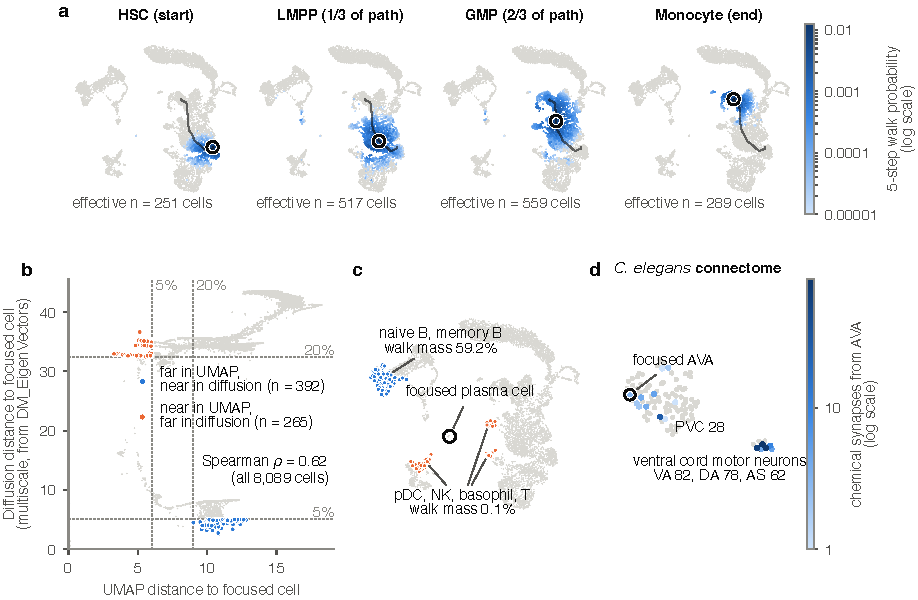
\includegraphics[width=\linewidth]{figures/fig2_cell_by_cell.pdf}
\caption{\textbf{A cell-by-cell matrix, read one focused cell at a time.}
\textbf{a}, The UMAP colored by the focused cell's row of a dense five-step diffusion walk (\texttt{obsp/\allowbreak diffusion\_walk\_t5}), for four cells along the shortest diffusion path from a hematopoietic stem cell (HSC) to a monocyte (line); the intermediates sit at one and two thirds of the path's diffusion length. Shared log scale; cells below $10^{-5}$ in gray. $n_\mathrm{eff} = 1/\sum p^2$ is the walk's effective number of cells. In AnnZarro each panel is one click.
%claim{fig2.plasma_rho} %claim{fig2.groups_def} %claim{fig2.groups_n}
\textbf{b}, For a focused plasma cell, UMAP distance against multiscale diffusion distance to every other cell (Spearman $\rho = 0.62$). Orange: among its 5\% nearest cells on the UMAP but outside its 20\% nearest in diffusion space (265 cells); blue: the reverse (392 cells).
%claim{fig2.walk_mass} %claim{fig2.dataset} %claim{fig2.knn} %claim{fig2.hsc_rho}
\textbf{c}, The same groups on the UMAP. Cells that look close (pDC, NK, basophil, T) receive 0.09\% of the plasma cell's walk mass; distant-looking naive and memory B cells receive 59.2\%. Across all 8,090 cells the UMAP preserves the global rank order of diffusion distances (median per-cell $\rho = 0.85$) but not local neighborhoods (median 14 of 30 nearest neighbors shared); the distortion concentrates in small, isolated populations, while the HSC-to-monocyte trajectory in \textbf{a} is faithful ($\rho = 0.95$ for the HSC). 
\textbf{d}, A connectome as a cell-by-cell matrix. \textit{C. elegans} neuron classes on a UMAP of their transcriptomes (CeNGEN\cite{taylor2021}, log TPM), colored by the focused class's row of chemical synapses (\texttt{obsp/\allowbreak chemical\_synapses}, synapses sent, summed over the neurons of each class\cite{varshney2011}; log scale), strongest on top; gray, no synapse from the focus. The command interneuron AVA sends its strongest output to the VA, DA and AS motor neurons, which sit in a separate cluster of the UMAP. }
\label{fig:cellcell}
\end{figure}}

\newcommand{\figgenegene}{%
\begin{figure}[p]
\centering
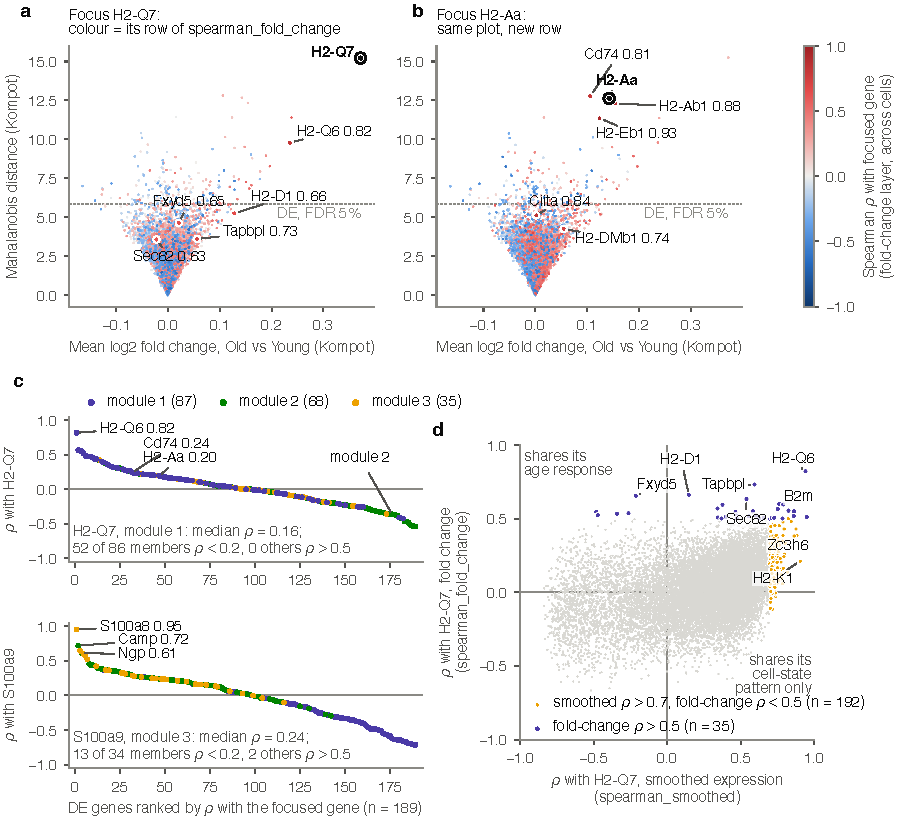
\includegraphics[width=\linewidth]{figures/fig3_gene_by_gene.pdf}
\caption{\textbf{A gene-by-gene matrix over a differential expression volcano.}
%claim{fig3.h2q7_partners} %claim{fig3.only_h2q6_de} %claim{fig3.fdr}
\textbf{a}, Kompot volcano (mean log$_2$ fold change against Mahalanobis distance, Old vs Young; dashed line, 5\% FDR) colored by the focused gene \textit{H2-Q7}'s row of the Spearman correlation of fold changes across cells (\texttt{varp/\allowbreak spearman\_fold\_change}). Its age response is shared by \textit{H2-Q6} ($\rho = 0.82$), \textit{Tapbpl} (0.73), \textit{H2-D1} (0.66) and \textit{B2m} (0.60), MHC class I antigen presentation; only \textit{H2-Q6} is itself called differentially expressed.
%claim{fig3.h2aa_partners}
\textbf{b}, The same plot after clicking \textit{H2-Aa} (histocompatibility 2, class II antigen A, alpha): the coloring follows the focus to MHC class II genes (\textit{H2-Eb1} 0.93, \textit{H2-Ab1} 0.88, \textit{Ciita} 0.84, \textit{Cd74} 0.81).
%claim{fig3.n_de} %claim{fig3.silhouette} %claim{fig3.module_mates} %claim{fig3.s100a9_partners}
\textbf{c}, Modules and focused rows. The 190 differentially expressed genes ranked by $\rho$ with \textit{H2-Q7} (top) or \textit{S100a9} (S100 calcium binding protein A9; bottom), colored, for comparison, by modules from average-linkage clustering of the same matrix on $1-\rho$ ($k = 3$, the silhouette maximum; silhouette is flat at 0.23--0.25 for $k = 2$--6). The rows show structure within and across modules: \textit{H2-Q7}'s module holds both MHC class I and class II genes, and 52 of its 86 module-mates have $\rho < 0.2$; \textit{S100a9}'s strongest partners Camp (0.72) and Ngp (0.61) fall outside its module, also at $k = 5$.
%claim{fig3.cell_state} %claim{fig3.h2k1}
\textbf{d}, \textit{H2-Q7}'s row of the correlation of smoothed expression against its row of the correlation of fold changes. 204 genes share its cell-state pattern ($\rho > 0.7$, smoothed), but only \textit{H2-Q6} also shares its age response; \textit{H2-K1} follows its expression pattern (0.90) but not its change with age (0.21). }
\label{fig:genegene}
\end{figure}}

\newcommand{\figcellgene}{%
\begin{figure}[p]
\centering
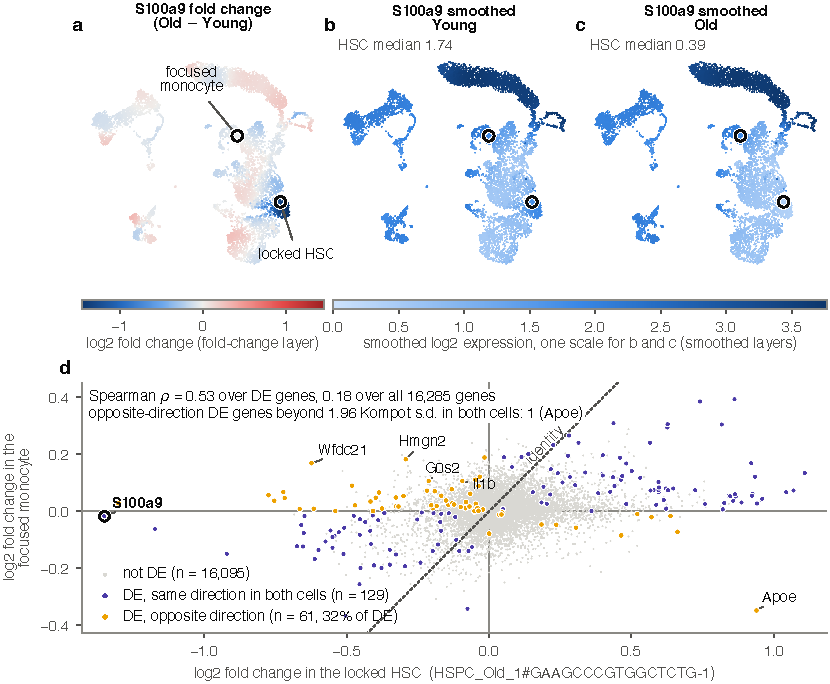
\includegraphics[width=\linewidth]{figures/fig4_cells_by_genes.pdf}
\caption{\textbf{Linking genes to cells and cells to genes.}
%claim{fig4.s100a9_mean} %claim{fig4.s100a9_hsc}
\textbf{a}, Focusing \textit{S100a9} colors the UMAP by its column of the Kompot fold-change layer. Its mean log$_2$ fold change is $-0.05$, so it looks unchanged in a volcano, yet it drops in hematopoietic stem cells (median $-1.35$; next lowest cell type $-0.21$).
%claim{fig4.s100a9_smoothed}
\textbf{b}, \textbf{c}, Its smoothed expression in Young and Old on one shared scale: HSC median 1.74 in Young and 0.39 in Old.
%claim{fig4.directions} %claim{fig4.beyond_sd} %claim{fig4.rows_rho} %claim{fig4.sd_cut}
\textbf{d}, Gene by gene, the fold-change row of a locked HSC against that of the focused monocyte (rings in \textbf{a}--\textbf{c}). Differentially expressed genes are colored by whether they change in the same (purple, 129) or opposite (amber, 61) direction in the two cells, with no magnitude cut. Opposite-direction changes are mostly small; beyond 1.96 times Kompot's per-cell standard deviation in both cells, only Apoe changes in opposite directions (up in the HSC, down in the monocyte), against 10 genes changing in the same direction. Spearman $\rho$ between the two rows is 0.53 over differentially expressed genes. }
\label{fig:cellgene}
\end{figure}}

\newcommand{\figperformance}{%
\begin{figure}[p]
\centering
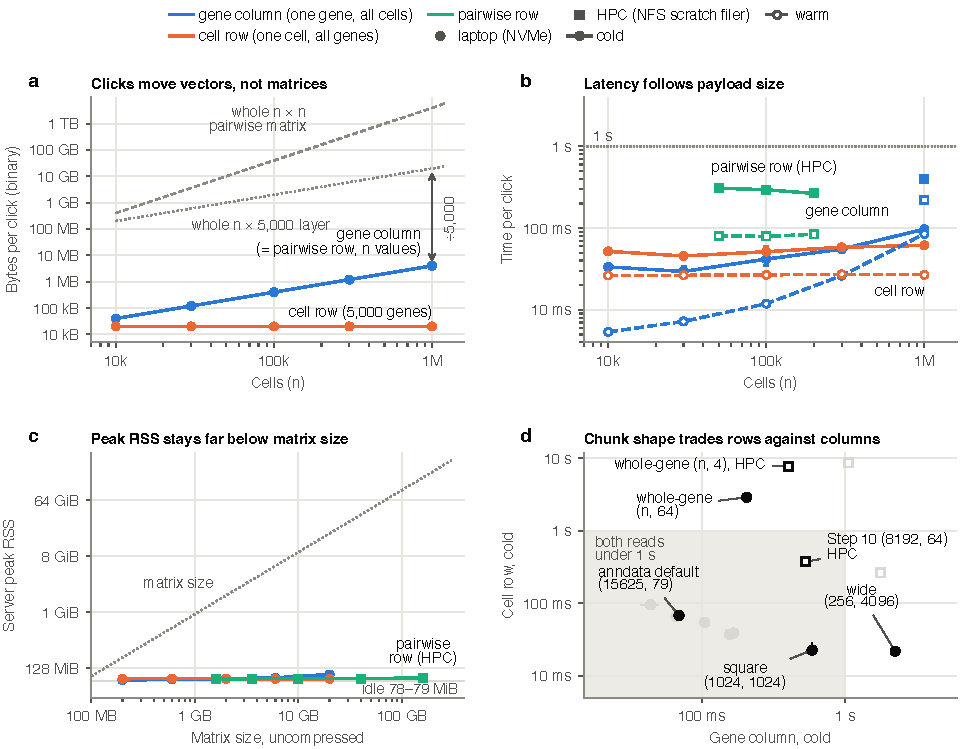
\includegraphics[width=\linewidth]{figures/fig6_performance.pdf}
\caption{\textbf{Interactions cost one vector, and memory stays flat.}
%claim{fig8.bytes} %claim{fig8.genes} %claim{fig8.bytes_per_value}
\textbf{a}, Bytes sent per click against the number of cells: a gene column, a cell row (5,000 genes) and a row of a dense pairwise matrix, with the size of the whole layer and the whole pairwise matrix for reference. Bytes are computed from the binary format, 4 bytes per float32 value, for the slices read in b (every value of these benchmark arrays is non-zero, so none is sent sparse). At one million cells a 20 GB layer is shown through a 4 MB gene column, one part in 5,000.
%claim{fig8.laptop_gene} %claim{fig8.hpc_gene} %claim{fig8.pairwise} %claim{fig8.hpc_node}
\textbf{b}, Latency per click on a laptop (M3 Max, NVMe), cold (filled) and warm (open; a new index). Gene columns stay under 1 s to one million cells on the laptop. On HPC nodes (Xeon Gold 6254, a whole 36-CPU node; data on $SCRATCH, an NFSv4.1 scratch filer), a gene column of a dense Tahoe-100M layer (whole-gene chunks) takes 0.40 s cold at 1 million cells, and a row of a dense 200,000~$\times$~200,000 matrix (160 GB uncompressed) 0.27 s cold; HPC points are squares.
%claim{fig8.peak_rss} %claim{fig8.idle} %claim{fig8.flat}
\textbf{c}, Peak resident memory of the server process against the uncompressed size of the matrix being read (dotted line, equality). On the laptop the server's peak stays at 82--102 MiB while the layer read grows a hundredfold, from 0.2 to 20 GB. A 160 GB pairwise matrix peaks at 89 MiB on HPC; the idle laptop server uses 79 MiB.
%claim{fig8.whole_gene} %claim{fig8.whole_gene_laptop}
\textbf{d}, Chunk shape trades cell-row against gene-column reads (one point per shape, cold). Whole-gene chunks make one cell row decompress the whole layer (2.9 s on the laptop at 1 million cells; 7.8 s on HPC); anndata's default chunks, like the aspect-ratio rule of Procedure Step 10, keep each read to a small part of the layer.
%claim{fig8.version}
Laptop series: AnnZarro 0.4.1 (the v0.4.1 tag, 78c9da6), vectors sent as binary float32. HPC series: the same tag on HPC nodes, cold meaning a fresh server with the node's page cache evicted.}
% Sources (paper repo, not cited in the text): benchmark/results/scale_v041.csv, sparse_v041.csv, sweep_v041.csv
\label{fig:performance}
\end{figure}}

% The figure takes a whole page; its caption follows as a separate float at the top of the next page.
\newcommand{\figscale}{%
\begin{figure}[p]
\centering
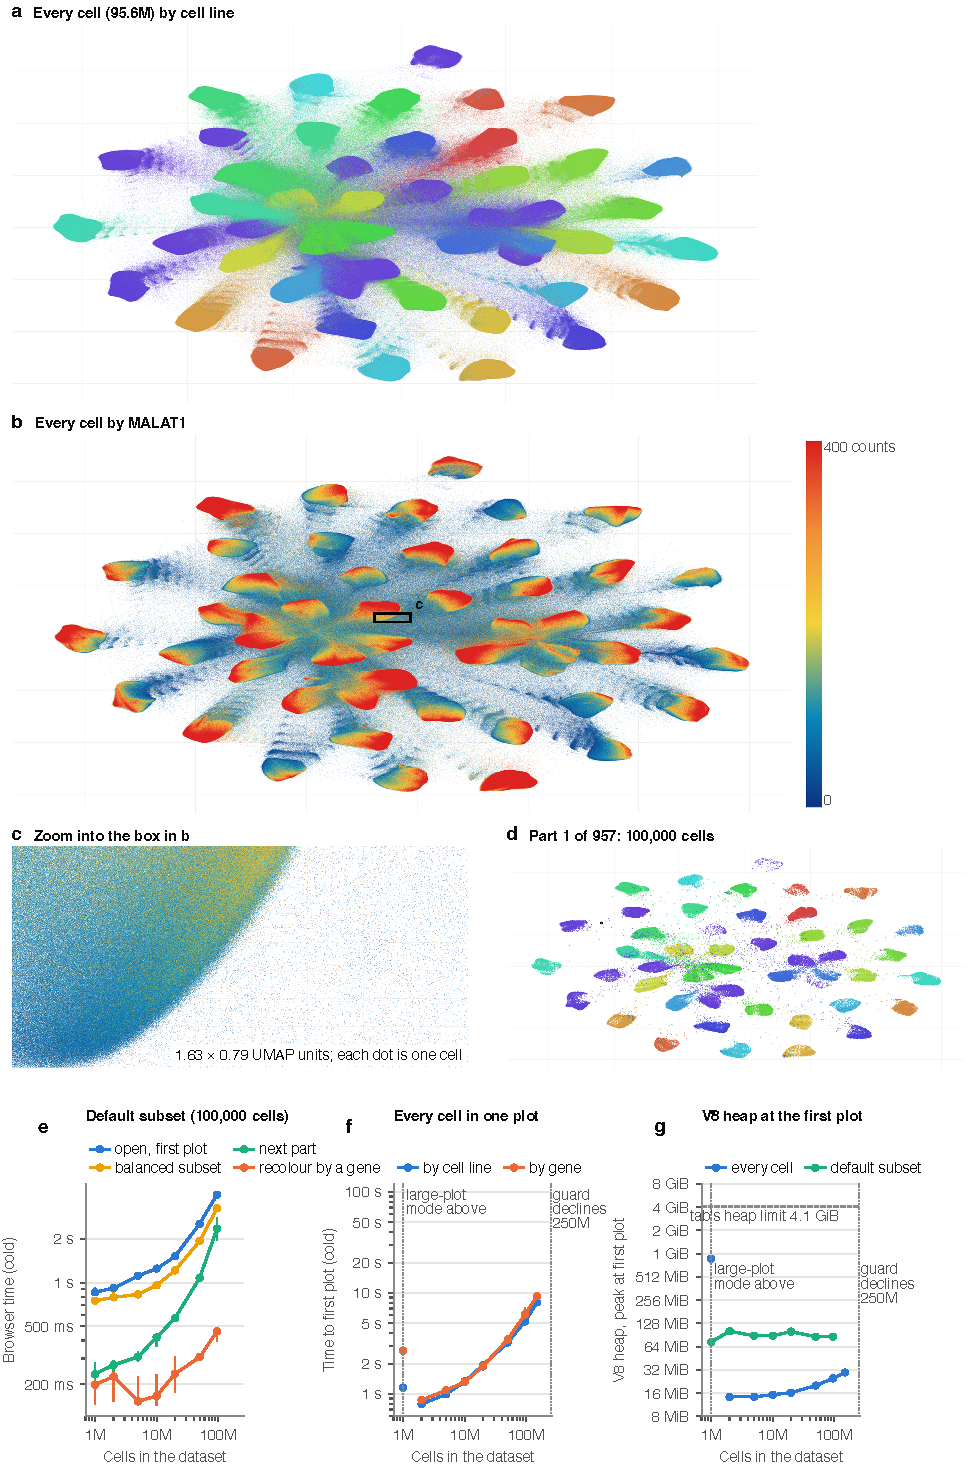
\includegraphics[width=\linewidth,height=\textheight,keepaspectratio]{figures/fig_scale.pdf}
\end{figure}
\begin{figure}[t]
\caption{\textbf{Tahoe-100M on a laptop: every cell in one plot, and a subset that stays interactive.}
%claim{fig7.n} %claim{fig7.machine}
All 95,624,334 cells of Tahoe-100M on a UMAP fitted to 999,073 reference cells and extended to every cell by nearest-neighbor placement (see \textit{Anticipated results}). Headless Chromium 153 on an Apple M3 Max laptop (128 GiB RAM); \textbf{a}--\textbf{d} show the plot areas of app screenshots.
% Sources (paper repo, not cited in the text): figures/scale
%claim{fig7a.time}
\textbf{a}, Every cell colored by cell line in large-plot mode, point size 1 and opacity 0.2; drawn 6.8 s after the page was opened in its screenshot session. In this mode the status line reads ``Large plot: no hover/click'', and its tooltip adds that table filters are off.
%claim{fig7b.cap}
\textbf{b}, The same cells colored by \textit{MALAT1} counts, the color scale running from 0 to 400 counts, which 97.9\% of cells do not exceed (6.8 s in its screenshot session). Where cells overlap, the highest values are drawn on top. The box marks the region shown in c.
%claim{fig7c.box} %claim{fig7c.style} %claim{fig7c.time}
\textbf{c}, The boxed region of b, $1.63 \times 0.79$ UMAP units at the edge of one cell line's island, where 96\% of the 574,309 cells belong to that line, opened zoomed from a view link with every cell drawn at the automatic point size and opacity (2.35 px and 0.43): each dot is one cell, colored on the scale of b (drawn in 17.6 s in its screenshot session). The link also focuses one cell; large-plot mode draws no focused-cell marker.
%claim{fig7d.part}
\textbf{d}, The default subset, part 1 of 957 (100,000 cells), in the regular plot with hover and focus, at the automatic size and opacity, over the same extent as a.
%claim{fig7e.range} %claim{fig7e.lines} %claim{fig7e.reps}
\textbf{e}, Browser time for actions on the default subset against dataset size, from 1 million cells (prefixes of Tahoe-100M) to all 95.6 million: opening to the first plot, recoloring by a gene, a subset balanced across the 50 cell lines and a step to the next part. Medians over 3 cold runs (2 events per run for recolor and part step), whiskers minimum to maximum; recolor and balanced subset start from a plot colored by a gene.
%claim{fig7f.rule_1M} %claim{fig7f.guard}
%claim{fig7f.tahoe_range}
\textbf{f}, Time to the first plot with every cell, colored by cell line or by a gene. Datasets up to 95.6 million cells are Tahoe-100M and its prefixes; the larger stores are described in \textbf{Supplementary Note~1}. The dotted rule at 1 million points marks the large-plot threshold: the plot at 1 million is regular, larger ones are drawn in large-plot mode; the dotted rule at 250 million marks where the memory guard declines the first plot at default settings, so larger stores are not shown.
% Sources (paper repo, not cited in the text): benchmark/tool_ceiling/ceilings.csv
%claim{fig7g.per_point}
\textbf{g}, Peak JavaScript (V8) heap at the first plot against the tab's heap limit under default Chromium flags (dashed line). The regular plot fills the heap fastest; large-plot mode keeps the positions off the heap (0.03 GiB at 150 million cells); the default subset stays flat.
% Sources (paper repo, not cited in the text): benchmark/scale/results/heapcap_v041.jsonl
% Times: browser_v041_events.csv (v0.4.1, tag 78c9da6); guard rule: ceilings.csv annzarro/v041; heap limit: heapcap_v041.jsonl; screenshot times: figures/scale/*.view.json (re-shot on v0.4.1, cd3e960).
}
\label{fig:scale}
\end{figure}}

\newcommand{\figapp}{%
\begin{figure}[p]
\centering
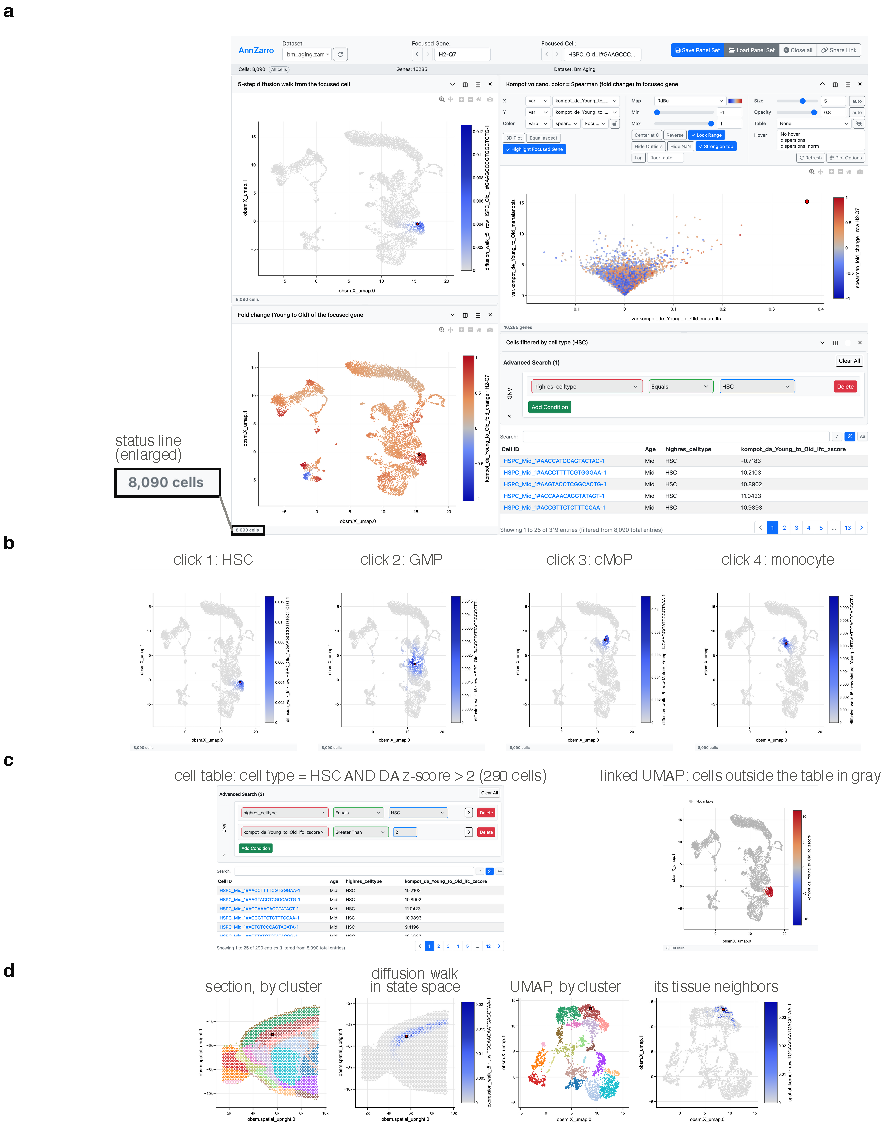
\includegraphics[width=\linewidth,height=541bp,keepaspectratio]{figures/fig5_app.pdf}% height cap: the page holds the figure and its caption; bp, not pt (541 pt = 539 bp printed the smallest text at 6.99 pt); tools/check_figures.py reads the printed size
\caption{\textbf{AnnZarro on the demonstration data.} \textbf{a}, Four linked panels with the focused gene \textit{H2-Q7} (histocompatibility 2, Q region locus 7) and a focused hematopoietic stem cell (header): the UMAP colored by the stem cell's row of a five-step diffusion walk; the Kompot volcano colored by each gene's fold-change correlation with \textit{H2-Q7}; the UMAP colored by \textit{H2-Q7}'s fold change; and a cell table filtered to stem cells. The volcano's controls are open, with \ui{Strong on top} pressed (the strongest values drawn last); the line under each plot is its status line (Step 34; inset, enlarged).
\textbf{b}, The diffusion-walk panel after four successive clicks from a stem cell through a granulocyte-monocyte progenitor (GMP) and a common monocyte progenitor (cMoP) to a monocyte; each click fetched one row.
%claim{fig5.filter}
\textbf{c}, A table filter combining two conditions (cell type is HSC and differential abundance z-score above 2; 290 of 8,090 cells) masks a linked UMAP: cells outside the table turn gray without any new data request. \textbf{d}, Mouse brain section profiled using Visium \cite{tenx_visium_mouse_brain_anterior} after a click on a cortex spot: the section by cluster; the spot's row of a diffusion walk in expression state space, which stays in its cortical layer without using tissue positions (%
%claim{figspatial.cortex_walk}
88.7\% of its mass falls in the spot's Leiden cluster); the UMAP by cluster and by the spot's row of a tissue-distance kernel.
% Sources (paper repo, not cited in the text): figures/numbers/app_spatial.json (2,693 spots, 2,000 highly variable genes, a five-step walk); data/spatial_demo.zarr from AnnZarro v0.4.1 docs/_tools/make_spatial_demo.py plus figures/spatial/add_expression_walk.py (obsp/expression_walk_t5 = row-normalized obsp/connectivities to the 5th power, as in Step 6); deep link figures/spatial_views/app_spatial_row4_cortex.view.json
}
\label{fig:app}
\end{figure}}


